\documentclass[12pt,a4paper]{article}
\usepackage[T2A]{fontenc}
\usepackage[utf8]{inputenc}
\usepackage[russian]{babel}
\usepackage[a4paper,left=2cm,right=2cm,top=2cm,bottom=2cm]{geometry}
\usepackage{amsmath,amssymb,amsthm,mathtools}
\usepackage{graphicx}
\usepackage{enumitem}
\usepackage[hidelinks]{hyperref}
\usepackage{indentfirst}

\setlist{itemsep=2pt,topsep=4pt}
\theoremstyle{plain}
\newtheorem{theorem}{Теорема}
\newtheorem{lemma}{Лемма}
\newtheorem{corollary}{Следствие}
\theoremstyle{definition}
\newtheorem{definition}{Определение}
\theoremstyle{remark}
\newtheorem*{remark}{Замечание}

\newcommand{\E}{\mathbb{E}}
\newcommand{\R}{\mathbb{R}}
\newcommand{\eps}{\varepsilon}
\newcommand{\norm}[1]{\left\lVert #1\right\rVert}
\newcommand{\abs}[1]{\left\lvert #1\right\rvert}
\newcommand{\ip}[2]{\left\langle #1,#2\right\rangle}

\begin{document}

\begin{center}
{\LARGE Безградиентная оптимизация\\[4pt] при липшицевом шуме}\\[10pt]
{\large Черновик результатов практикума}\\[8pt]
Фролов Александр\\[2pt]
{\small ноябрь 2026; код и эксперименты~--- репозиторий \texttt{lipnoise-zo}}
\end{center}

\noindent\textbf{Цель:} найти, какой неслучайный шум в значениях функции допускает двухточечный безградиентный метод для \emph{негладких} выпуклых задач, если шум имеет липшицеву структуру, и доказать, что найденный порог неулучшаем.

\medskip
\noindent\textbf{Коротко.} Для выпуклой $M_f$-липшицевой задачи на множестве диаметра $D$ шум, представимый в виде суммы $M$-липшицевой функции и функции с колебанием не больше $\Delta_0$, допустим тогда и только тогда (с точностью до констант и логарифмов), когда
\begin{equation}\label{eq:region}
  M\lesssim\frac\eps D\qquad\text{и}\qquad\Delta_0\lesssim\frac{\eps^2}{\sqrt d\,M_fD},
\end{equation}
причём \textbf{амплитуда шума может быть любой}. Липшицева часть допустима на уровне $\Theta(\eps/D)$ без зависимости от размерности.

\medskip
\noindent\textbf{Положение в литературе} (подробно~--- раздел~\ref{sec:lit}). Для функций с ограниченным гессианом точный порог $\Theta(\eps/R)$ доказан в~\cite{LDT26}. Для негладкого двухточечного случая в~\cite{DTTG23} получено $\eps/(D\sqrt d)$ с гипотезой, что этот порог точен. Наш вклад скромный: мы показываем, что и в негладком случае порог равен $\Theta(\eps/D)$, то есть множитель $\sqrt d$ в~\cite{DTTG23}~--- артефакт анализа, и добавляем скачки $\Delta_0$, зависящие от $x$, и эксперименты с округлением. Технически это сочетание известных приёмов.

\section{Постановка}

$Q\subset\R^d$~--- выпуклое замкнутое множество диаметра $D$; $f:\R^d\to\R$ выпукла и $M_f$-липшицева; $f^*=\min_Qf$. Оракул на запрос $x\in\R^d$ возвращает $\tilde f(x)=f(x)+\delta(x)$, где $\delta$~--- детерминированная функция, зафиксированная до запуска (шум не зависит от случайности метода).

\begin{definition}
Шум принадлежит классу $\mathcal N(M,\Delta_0)$, если
\begin{equation}\label{eq:class}
  \abs{\delta(x)-\delta(y)}\le\Delta_0+M\norm{x-y}\qquad\forall x,y\in\R^d .
\end{equation}
\end{definition}
Частные случаи: $\mathcal N(0,2\Delta)$ содержит любой шум с $\abs\delta\le\Delta$ (ограниченный враждебный шум); $\mathcal N(M,0)$~--- $M$-липшицевы функции (амплитуда не ограничена); округление значений до сетки шага $q$ лежит в $\mathcal N(0,q)$. Модель~\cite[разд.~4]{GDN16}~--- липшицева часть плюс часть, не зависящая от $x$,~--- частный случай с $\Delta_0=0$ после сокращения в разности.

\textbf{Метод.} Проекционный двухточечный ZO-SGD: $e_k\sim\mathrm{Unif}(S^{d-1})$,
\begin{equation}\label{eq:method}
  g_k=\frac d{2\gamma}\bigl(\tilde f(x_k+\gamma e_k)-\tilde f(x_k-\gamma e_k)\bigr)e_k,\qquad x_{k+1}=\Pi_Q(x_k-hg_k),\qquad\bar x_N=\frac1N\sum_{k=0}^{N-1}x_k .
\end{equation}

\section{Структура шума и свойства оценки}

\begin{lemma}[разложение]\label{lem:decomp}
Пусть $\delta\in\mathcal N(M,\Delta_0)$ и $\delta_L(x)=\inf_y\bigl[\delta(y)+M\norm{x-y}\bigr]$. Тогда $\delta_L$ $M$-липшицева и $0\le\delta-\delta_L\le\Delta_0$. Обратно, сумма $M$-липшицевой функции и функции со значениями в $[0,\Delta_0]$ лежит в $\mathcal N(M,\Delta_0)$.
\end{lemma}
\begin{proof}
Подстановка $y=x$ даёт $\delta_L\le\delta$. По~\eqref{eq:class} $\delta(y)+M\norm{x-y}\ge\delta(x)-\Delta_0$ для всех $y$, откуда $\delta_L\ge\delta-\Delta_0>-\infty$. Нижняя грань семейства $M$-липшицевых функций $x\mapsto\delta(y)+M\norm{x-y}$, конечная хотя бы в одной точке, $M$-липшицева. Обратное утверждение очевидно.
\end{proof}

Обозначим $h_\gamma(x)=\E_uh(x+\gamma u)$, $u\sim\mathrm{Unif}(B^d)$. Для непрерывной $h$ по формуле Стокса $\nabla h_\gamma(x)=\frac d\gamma\E_e[h(x+\gamma e)e]$, и если $h$ $M$-липшицева, то $h_\gamma$ тоже $M$-липшицева, поэтому $\norm{\nabla h_\gamma}\le M$.

\begin{lemma}[смещение и второй момент]\label{lem:bias}
Пусть $\delta\in\mathcal N(M,\Delta_0)$, $d\ge2$, и $g$~--- оценка~\eqref{eq:method} в точке $x$. Тогда
\begin{equation}\label{eq:bias}
  \E_eg=\nabla f_\gamma(x)+b(x),\qquad\norm{b(x)}\le M+\frac{\sqrt d\,\Delta_0}{2\gamma},
\end{equation}
\begin{equation}\label{eq:moment}
  \E_e\norm g^2\le4d(M_f+M)^2+\frac{d^2\Delta_0^2}{2\gamma^2}.
\end{equation}
\end{lemma}
\begin{proof}
Разложим $\delta=\delta_L+\delta_B$ по лемме~\ref{lem:decomp}, $\delta_B\in[0,\Delta_0]$. По формуле Стокса (в симметризованном виде) часть оценки, порождённая $f+\delta_L$, имеет среднее $\nabla f_\gamma+\nabla(\delta_L)_\gamma$, и $\norm{\nabla(\delta_L)_\gamma}\le M$. Для части $\beta$, порождённой $\delta_B$, при единичном $r$, так как $\abs{\delta_B(a)-\delta_B(b)}\le\Delta_0$ и $\E\abs{\ip er}\le1/\sqrt d$,
\[
  \ip{\E\beta}r\le\frac d{2\gamma}\Delta_0\,\E\abs{\ip er}\le\frac{\sqrt d\Delta_0}{2\gamma}.
\]
Для второго момента $\norm g^2\le2\norm{g_1}^2+2\norm{g_2}^2$, где $g_1$ порождена $f+\delta_L$, а $g_2$~--- $\delta_B$. Функция $\varphi(e)=(f+\delta_L)(x+\gamma e)$ является $\gamma(M_f+M)$-липшицевой на сфере, и по неравенству Пуанкаре $\E\norm{g_1}^2\le\frac{d^2}{4\gamma^2}\cdot\frac{4\gamma^2(M_f+M)^2}{d-1}\le2d(M_f+M)^2$. Наконец, $\norm{g_2}^2\le\frac{d^2\Delta_0^2}{4\gamma^2}$.
\end{proof}

\begin{remark}
Смещение от липшицевой части не содержит ни $\sqrt d$, ни деления на $\gamma$, тогда как ограниченный шум даёт $\sqrt d\Delta_0/\gamma$. Численная проверка~--- эксперимент E1 и тесты в \texttt{tests/test\_theory.py}.
\end{remark}

\section{Верхняя оценка}

\begin{theorem}\label{th:upper}
Пусть $\eps\le M_fD$, $\gamma=\eps/(3M_f)$, $h=D/(G\sqrt N)$ с $G^2=5d(M_f+M)^2$, и шум $\delta\in\mathcal N(M,\Delta_0)$ удовлетворяет
\begin{equation}\label{eq:upper-cond}
  M\le\frac{\eps}{6D},\qquad\Delta_0\le\frac{\eps^2}{9\sqrt d\,M_fD}.
\end{equation}
Тогда метод~\eqref{eq:method} после $N=\lceil45\,d(M_f+M)^2D^2/\eps^2\rceil$ итераций, то есть $T=2N$ вызовов оракула, выдаёт $\bar x_N\in Q$ с $\E f(\bar x_N)-f^*\le\eps$. Амплитуда шума в условия не входит.
\end{theorem}
\begin{proof}
По~\eqref{eq:upper-cond} и $\eps\le M_fD$ имеем $\frac{d^2\Delta_0^2}{2\gamma^2}\le\frac{d\eps^2}{18D^2}\le d(M_f+M)^2$, поэтому по~\eqref{eq:moment} $\E\norm{g_k}^2\le G^2$. По~\eqref{eq:bias} $\norm{b}\le\frac\eps{6D}+\frac{\sqrt d\Delta_0}{2\gamma}\le\frac\eps{3D}=:B$. Применим основное неравенство для проекционного SGD со смещённым градиентом (методичка, утверждение~3.1) к выпуклой дифференцируемой функции $f_\gamma$ на $Q$ с минимумом $x^*_\gamma$: при $h=D/(G\sqrt N)$
\[
  \E f_\gamma(\bar x_N)-f_\gamma(x^*_\gamma)\le\frac{DG}{\sqrt N}+BD\le\frac\eps3+\frac\eps3 .
\]
Наконец, $f\le f_\gamma$ (Йенсен) и $f_\gamma(x^*_\gamma)\le f_\gamma(x^*)\le f^*+\gamma M_f=f^*+\eps/3$.
\end{proof}

\begin{remark}
Число вызовов $T=O(d(M_f+M)^2D^2/\eps^2)$ оптимально по $d$ и $\eps$ (Duchi et al.\ 2015). Следующий шаг~--- батчированный ускоренный вариант с $N=O(d^{1/4}M_fD/\eps)$ раундов; для него нужна теорема об устойчивости ускоренного метода к аддитивному смещению при ограниченной траектории (методичка, §4.4).
\end{remark}

\section{Нижняя оценка по липшицевой части}

\begin{theorem}\label{th:lower}
Пусть $Q$~--- шар радиуса $\rho=D/2$ с центром в нуле, $\eps<M_f\rho$, и $M>2\eps/D$. Тогда для любого (рандомизированного, адаптивного) алгоритма с любым числом запросов в любых точках $\R^d$ найдутся выпуклая $M_f$-липшицева $f$ и шум $\delta\in\mathcal N(M,0)$, при которых $\E f(\hat x)-f^*>\eps$ для выхода $\hat x\in Q$.
\end{theorem}
\begin{proof}
Возьмём $a\in(2\eps/D,\min\{M,M_f\}]$, единичный $u$ и $f_\pm(x)=\pm a\ip ux$, $\delta_\pm=-f_\pm$. Шум $a$-липшицев, оракул в обоих случаях всегда отвечает нулём, поэтому распределение $\hat x$ одинаково. Так как $\min_Qf_\pm=-a\rho$,
\[
  \E[f_+(\hat x)-f_+^*]+\E[f_-(\hat x)-f_-^*]=\E\bigl[a\ip u{\hat x}+a\rho-a\ip u{\hat x}+a\rho\bigr]=aD>2\eps,
\]
и одно из слагаемых больше $\eps$.
\end{proof}

\begin{corollary}
Допустимый уровень липшицевой части равен $\Theta(\eps/D)$: теоремы~\ref{th:upper} и~\ref{th:lower} расходятся лишь в константе $12$, и порог не зависит от $d$ и от амплитуды. Для ограниченной части при $M=0$ нижняя оценка Ристески--Ли $\Delta_{\max}\lesssim\max\{\eps^2/(\sqrt dM_fD),\eps/d\}$ (с точностью до логарифмов) показывает, что условие на $\Delta_0$ в~\eqref{eq:upper-cond} неулучшаемо при не слишком малых $\eps$. Поэтому область~\eqref{eq:region} точна по обеим осям.
\end{corollary}

\begin{remark}
Принадлежность классу не единственна: шум малой амплитуды $\Delta$ лежит и в $\mathcal N(0,2\Delta)$. Поэтому для «рампы» высоты $\Delta$ и наклона $M$ шум безвреден, если \emph{либо} $M\lesssim\eps/D$, \emph{либо} $\Delta\lesssim\eps^2/(\sqrt dM_fD)$: область безвредности в плоскости $(\Delta,M)$ имеет форму буквы «Г». Это видно в эксперименте E2.
\end{remark}

\section{Связь с литературой}\label{sec:lit}

\begin{itemize}
  \item \cite[разд.~4]{GDN16} (2016): шум~--- липшицева часть плюс часть, не зависящая от $x$; двухточечная схема; допустимость $\delta=O(\eps)$ выведена из условия $\norm{\nabla\E\delta(x+\tau\tilde s)}=O(\eps/R)$, то есть по сути из того же наблюдения, что и лемма~\ref{lem:bias}. Число вызовов $n^2M^2R^2/\eps^2$, оптимальность оставлена открытой (сноска 46).
  \item \cite{DTTG23}: негладкие выпуклые и седловые задачи, двухточечная схема, $M_\delta$-липшицев шум (Assumption~2.3). Смещение оценено как $\sqrt d\,M_\delta$ (формула (62)), поэтому допустимо $M_\delta\lesssim\eps/(D\sqrt d)$. В приложении~B доказано лишь $M_{\max}\lesssim\eps/D$ (при дополнительных предположениях), и авторы пишут, что считают точным порог $\eps/(D\sqrt d)$.
  \item \cite{LDT26} (октябрь 2026): функции гёльдеровой гладкости $\beta>2$ с ограниченным гессианом. Систематическая $M$-липшицева ошибка: для сильно выпуклых $M_{\max}=\Theta(\sqrt{\alpha\eps})$, для выпуклых $\eps/(16R)\le M_{\max}\le2\eps/R$ (теорема~5(b)); нижняя оценка~--- та же пара линейных функций, что в теореме~\ref{th:lower} (лемма~E.7). Верхняя оценка использует $L<\infty$.
\end{itemize}

\textbf{Что здесь нового.} (1) Точный порог $\Theta(\eps/D)$ для негладких функций в двухточечной схеме с оптимальным числом вызовов $O(dM_f^2D^2/\eps^2)$: это закрывает зазор $\sqrt d$ из~\cite{DTTG23} и опровергает их гипотезу; (2) класс $\mathcal N(M,\Delta_0)$ со скачками, зависящими от $x$, и Г-образная область безвредности; (3) эксперименты, в частности «мёртвая зона» при округлении. Пункты (1)--(2)~--- аккуратная заметка; пункт (3) пока без теории.

\section{Эксперименты}

Код: \texttt{lipzo/} (модели шума, оценка, метод), \texttt{tests/} (6 проверок лемм, 15 тестов), \texttt{experiments/} (воспроизведение одной командой \texttt{bash run\_all.sh}).

\paragraph{E1. Смещение в зависимости от размерности.} Шум направлен вдоль одной оси, поэтому среднее оценки вычисляется точно одномерной квадратурой (без Монте-Карло). Ступенька высоты $2\Delta$ даёт смещение, растущее как $\sqrt{2d/\pi}\,\Delta/\gamma$; липшицева рампа даёт смещение, ограниченное наклоном $M$ при всех $d$ (при $d\ge128$ отношение к $M$ равно $1{,}000$).

\begin{center}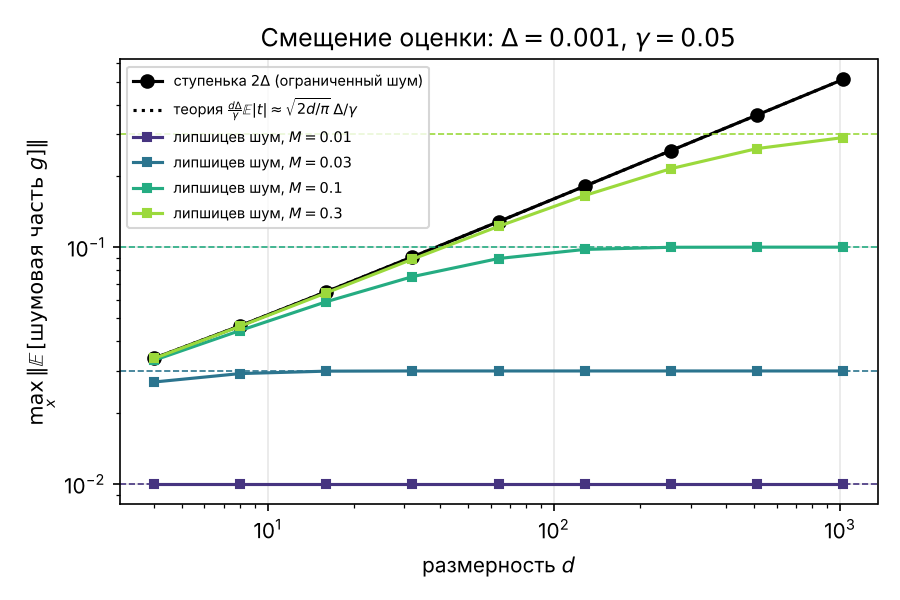
\includegraphics[width=0.78\textwidth]{../results/e1_bias.png}\end{center}

\paragraph{E2. Фазовый переход в плоскости $(\Delta,M)$.} Постановка слайда~29 доклада: $f(x)=-g_0\ip ux$ на единичном шаре, $g_0=2\eps/R$, $\eps=0{,}1$, шум~--- «стена» поперёк гиперплоскости $\ip ux=0$, старт $x_0=-0{,}6u$, $d=20$, $\gamma=0{,}05$, 3000 итераций, 16 запусков на клетку. Предсказание «метод блокируется $\iff$ максимальное смещение больше $g_0$» совпадает с экспериментом в $97{,}6\%$ клеток. Расхождения~--- столбец $M\approx0{,}16$ чуть ниже порога $g_0=0{,}2$: там стена не блокирует, а замедляет метод (суммарный наклон $0{,}04$), и при $10^4$ итерациях все запуски успешны; при $M=0{,}25>g_0$ неудача сохраняется при любом бюджете.

\begin{center}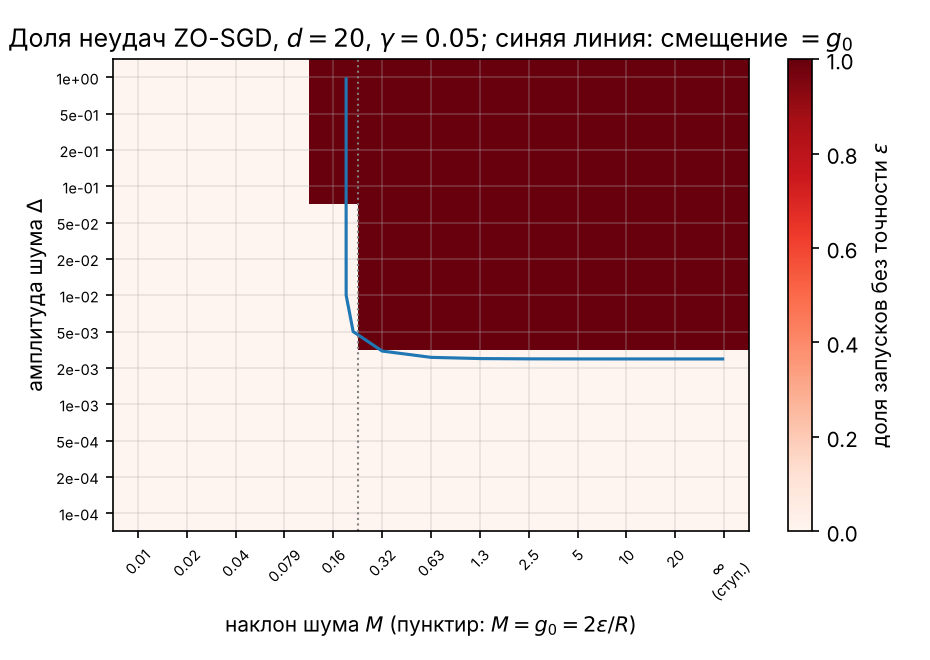
\includegraphics[width=0.78\textwidth]{../results/e2_phase.png}\end{center}

\paragraph{E3. Реальное округление.} $f(x)=1+\norm{x-c}_1/\sqrt d$ ($M_f=1$), $d=10$, $2\cdot10^4$ итераций; значения вычисляются в fp64, fp32, bf16, fp16 и fp16 со стохастическим округлением (случайный последний бит, как в~\cite[разд.~4]{GDN16}). Наблюдения:
\begin{enumerate}
  \item Оценка худшего случая $M_f\gamma+D\sqrt d\Delta_0/(2\gamma)$ (пунктир) пессимистична на 2--3 порядка: при достаточно большом $\gamma$ округление практически безвредно.
  \item При малом $\gamma$ механизм отказа другой: значения в $x\pm\gamma e$ округляются в одно число, оценка равна нулю, и метод стоит на месте («мёртвая зона»). Порог по $\gamma$ у bf16 в $8=2^3$ раза больше, чем у fp16~--- ровно разница мантисс; порядок порога $\gamma\sim\sqrt d\,\mathrm{ulp}/M_f$.
  \item Стохастическое округление сдвигает мёртвую зону примерно втрое и снижает итоговую ошибку; при совсем малых $\gamma$ мешает уже дисперсия $d^2q^2/\gamma^2$.
\end{enumerate}

\begin{center}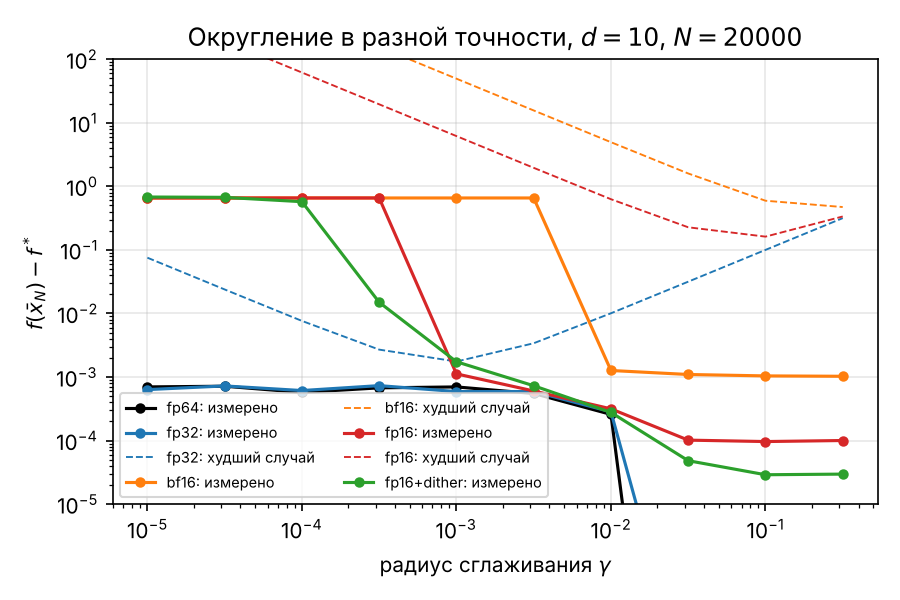
\includegraphics[width=0.78\textwidth]{../results/e3_rounding.png}\end{center}

\section{Следующие шаги и вопросы}

\begin{enumerate}
  \item Ускоренный батчированный вариант теоремы~\ref{th:upper} (три критерия: $T$, $N$, допустимый шум).
  \item Модель округления: доказать порог мёртвой зоны $\gamma\gtrsim\sqrt d\,q/M_f$ и оценку для случайного (не враждебного) округления, объясняющую E3.
  \item Шум, зависящий от истории запросов: верна ли теорема~\ref{th:upper}, если липшицевость требуется только при фиксированной истории?
  \item Формализация теоремы~\ref{th:upper} в LongTails. Основа~--- готовый Setup

  \texttt{AdaptivePairedZerothOrder}, в котором условие $\abs\delta\le\Delta$ заменяется на~\eqref{eq:class}.
\end{enumerate}

\textbf{Вопросы к А.\,В.~Гасникову:} (1) какая модель липшицева шума имелась в виду; (2) стоит ли оформить негладкий случай как короткую заметку или сразу двигаться к продолжению (теория округления, ускорение, шум, зависящий от истории); (3) нужен ли «кубик» адаптивности; (4) допустимо ли использовать LongTails в курсовой работе.

\begin{thebibliography}{9}
\bibitem{GDN16} А.\,В.~Гасников, П.\,Е.~Двуреченский, Ю.\,Е.~Нестеров. Стохастические градиентные методы с неточным оракулом. arXiv:1411.4218 (2016).
\bibitem{survey} A.~Gasnikov et al. Randomized gradient-free methods in convex optimization. arXiv:2211.13566.
\bibitem{duchi} J.~Duchi, M.~Jordan, M.~Wainwright, A.~Wibisono. Optimal rates for zero-order convex optimization: the power of two function evaluations. IEEE Trans.\ Inf.\ Theory, 2015.
\bibitem{rl} A.~Risteski, Y.~Li. Algorithms and matching lower bounds for approximately-convex optimization. NeurIPS 2016.
\bibitem{DTTG23} D.~Dvinskikh, V.~Tominin, Y.~Tominin, A.~Gasnikov. Gradient-free optimization for non-smooth minimax problems with maximum value of adversarial noise. arXiv:2202.06114 (v3, 2023).
\bibitem{LDT26} T.~Loginov, D.~Dvinskikh, N.~Tupitsa, O.~Osmanov, Y.~Dorn, A.~Gasnikov. Minimax oracle call complexity, rounds and admissible noise in zeroth-order optimization of highly smooth functions. arXiv:2610.05517 (2026).
\end{thebibliography}

\end{document}
